\subsection{Filtertype}
\label{Filtertype}
%
Hvis der kun fokuseres på de filtre der skal forstærke de lave frekvenser, vil det være nødvendigt at konstruere filtrene som lavpasfiltre. Et normalt første ordens lavpasfilter har en hældning på -20dB/dek, men da kravet er at filtrene skal kunne forstærke med 2.62dB mellem 20Hz og 1000Hz, er det ikke muligt at udvikle filtrene, som første ordens lavpasfiltre, de skal derimod konstrueres som fraktal ordens filtre. 
%
\begin{figure}[H]
	\centering
	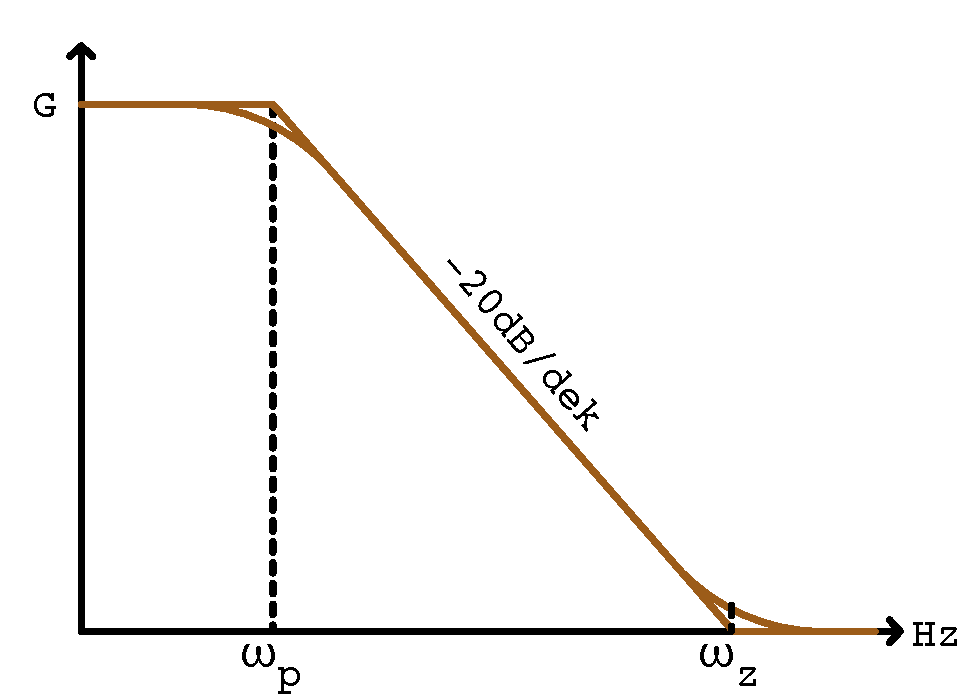
\includegraphics[resolution=300,scale=\circuitSize]{Figure/DesignAfFilter/FoersteordensFilter.pdf}
	\caption{Hældningen for et første ordens lavpasfilter.}
	\label{fig:1OrdensFilter}
\end{figure}
\noindent
%
På \autoref{fig:1OrdensFilter} illustreres hældningen per dekade for et første ordens lavpasfilter med tilhørende pol, $\omega_p$ og nulpunkt, $\omega_z$. Overføringsfunktionen for et første ordens lavpasfilter, er som følger:
%
\begin{equation}
	H(s) = \frac{G*\left(1+\frac{s}{\omega_z}\right)}{\left(1+\frac{s}{\omega_p}\right)}
\end{equation}  
%
$G$ angiver forstærkningen. For at få en hældning på -20dB/dek ved et første ordens filter gælder følgende forhold mellem pol- og nulpunkt:
%
\begin{equation}
	\frac{\omega_z}{\omega_p} > 10
\end{equation} 
%
Hvorimod hvis der skal forstærkes med mindre end -20dB/dek gælder det at:
%
\begin{equation}
	\frac{\omega_z}{\omega_p} < 10
\end{equation}
%
Da filtre generelt angiver en forstærkning eller dæmpning per dekade, er det nødvendigt at beregne hvor meget en forstærkning på 2.62dB mellem 20Hz og 1000Hz vil svarer til per dekade, først beregnes dekaden:
%
\begin{equation}
	log_{10}\left(\frac{1000Hz}{20Hz}\right) = 1.699dek
\end{equation}
%
Så kan forstærkningen per dekade beregnes: 
%
\begin{equation}
	\frac{2.62dB}{1.699dek} = 1.5421dB/dek
\end{equation}
%
Da der både udvikles filtre der forstærker og dæmper vil forstærkningen være $\pm$1.5421dB/dek. 

Ved lave hældninger over et større frekvens område, kan det blive nødvendigt at tilføje flere pol/nulpunkt par. I følgende afsnit vil det blive undersøgt hvor mange af disse par, der er nødvendige for at få den korrekte forstærkning. 